\chapter{Methods}

\section{Caries detection - baseline model comparison}

Firstly we implemented and tested multiple object-detection architectures. We compared them against each other on the stage of the dataset that was currently available.

\subsection{Dataset}
We used the first five stages of the dataset mentioned in chapter \ref{chapter:dataset}. The dataset was always split into train, validation and test parts. Each of them consising of 70\%, 15\%, and 15\% of the dataset.

\subsection{Image augmentations}
The image was augmented by a single pipeline that applied the following transformations with corresponding probabilities p.
\begin{itemize}
    \item Normalize by substracting the mean of the dataset and dividing by standard deviation of the dataset (mean$=0.37$, std$=0.28$), $p=1$
    \item Resize and pad to $1024\times1024/896$, $p=1$
    \item Horizontal flip, $p=0.5$
    \item Vertical flip, $p=0.5$
    \item Rotation, $p=0.3$, rotation limit$=10^{\circ}$
    \item Translation, $p=0.5$, translation limit$=10\%$ of the image size
    \item Gaussian blur flip, $p=0.3$, kernel size from 7 to 31
    \item Gamma correction, $p=0.3$, $\gamma$ in range from 0.6 to 1.4
\end{itemize}
The result of those augmentations can be seen in the appendix \ref{appendix:img_transformations}.

The dimensions to which resize an image were selected due to limitations of some architectures, which require the input to be divisible by 128. In the beginning, we used square images, due to the ease of implementation. We swithched to rectangular images after that, but no improvement on measured metrics was observed. Based on the architecture, we observed a decrease in GPU memory usage in the range from 5\% to 10\%.

\subsubsection{Computing power}
All the computations were realized on the CMP cluster, consisting of multiple GPU nodes. The experiments were conducted on the Boruvka and Zorn machines. Both of them have 32 CPU cores, 256GB of RAM memory, and 8 NVIDIA GeForce GTX 1080-Ti graphics cards with 12GB of dedicated memory.

\subsection{Neural network models}
\label{sec:methods:nns}
Multiple architectures of neural networks were used. As the work on the thesis progressed, the amount grew larger; thus on the advanced stages of the dataset, a wider variety of models can be seen. We stopped using the YOLOv3 model after stage 2, since the YOLOv5 model has superior performance on stages one and two.

All the models we used and their respective backbones are listed bellow
\begin{itemize}
    \item YOLOv3 with Darknet-53 backbone
    \item YOLOv5 with backbones with the sixth generation of backbones. We used the small, medium, large and extra lasrge vesions of those backbones. In the further text, we will denote them as s6, m6, l6, x6.
    \item Faster-RCNN with Resnet50 and Resnet101 backbone. R50 and R101 abbreviations will be used for those.
    \item RetinaNet with Resnet50 and tiny swin transformer (swint) Backbones.
    \item EfficientDet with D0,D1,D2,D3,D4 and D5 backbones
\end{itemize}

\subsubsection{Batch-size}
The batch size differed based on the model architecture and selected backone. We always used the biggest batch size that was able to fit into the graphics card memory. An overview of batch sizes for a different combination of architectures and backbones is in table TODO. Note that those batch size values allow for the accumulation of 4 forward passes into the GPU memory.

\begin{table}
    \centering
    \begin{tabular}{|c|c|c|c|}
        \hline
        model-backbone  & batch size & model-backbone   & batch size \\ \hline
        YOLOv5-s6       & 16         & EfficientDet-D0  & 5          \\ \hline
        YOLOv5-m6       & 8          & EfficientDet-D1  & 4          \\ \hline
        YOLOv5-l6       & 4          & EfficientDet-D2  & 3          \\ \hline
        YOLOv5-x6       & 2          & EfficientDet-D3  & 2          \\ \hline
        FRCNN-R50       & 2          & EfficientDet-D4  & 1          \\ \hline
        FRCNN-R101      & 5          & EfficientDet-D5  & 1          \\ \hline
        RetinaNet-swint & 3          & YOLOv3 - Darknet & 4          \\ \hline
        RetinaNet-R50   & 4          & -                & -          \\ \hline
    \end{tabular}
    \caption{Maximal batch sizes, that fit into 12GB GPU for a given model}
    \label{tab:batch_sizes}
\end{table}



\subsubsection{Optimizers}
The Adam optimizer was used during all experiments. The parameters $\beta_1, \beta_2$ were set to 0.9 and 0.999 and weight decay was chosen to be $10^{-6}$. Since we could not fit reasonably big batch sizes into the GPU, the optimization step was performed every four forward passes. This should emulate a bigger batch size and increase the chance of finding global optimization minima.

\subsubsection{Learning rate}
We initialy experimented with different learinig rates and used the learning rate test to find the initial learning rate. In the end, there was no difference in the final performance of the model, and the number of epochs required to train the model did not differ significantly. In rare cases, the learning rate test's learning rate did not leadd to model convergence. We, therefore, set the initial learning rate to $10^{-4}$ and used a reduced on plateau learning rate scheduler. The monitored value by the scheduler was validation loss, and the learning rate decreased by a factor of 5 when the improvement of the loss stalled for five consecutive epochs.
\subsubsection{Termination condition}
The training was halted when the $AP@.5$ did not increase throughout 10 epochs, but not earlier than after 50 epochs from the beginning of the training.

\section{Caries detection - model improvements}
\subsection{General changes}
\label{sec:general_changes}
We replaced the Adam optimizer with AdamW with the same $\beta_1$ and $\beta_2$. Furthermore, a cosine annealing learning rate scheduler was used. The half-period of cosine was set to 70 epochs and the minimal learning rate to $10^{-7}$.
Multiple models from section \ref{sec:methods:nns} were used and the training was done on stage five dataset.
\subsection{Group normalization}


\section{Model instpection}
We conducted several experiments to asses model behavior. All experiments were made on dataset made in fifth stage with models, whose results are in tables \ref{tab:improved:precision}, \ref{tab:improved:recall},\ref{tab:imrpoved:prf}.
\subsection{Size of backbone}
We explored the influence of the backbone choice on the performance of the model. We therefore used YOLOv5 model and trained it multiple times with small, medium and large backbone. The training was done by the approach described in sections this section including improvements mentioned in subsection \ref{sec:general_changes}.

\subsection{Weight decay}
We experimented with different values of weight decay. We used Faster-RCNN architecture with ResNet50 backbone and YOLOv5 with medium size backbone and tried the following values of weight decay: $10^{-2}, 10^{-4}, 10^{-6}, 10^{-8}$.

\section{Dental-restorations segmentation segmentation}
\subsection{Non-deeplearning approach}
We decided to test the approach that Abdalla-Aslan proposed, and Yeshua \cite{AbdallaAslan2020, Yeshua2019} as described in section \ref{sec:related_works:dental_restorations}. This means that we defined a pipeline of image processing operations, where we:
\begin{itemize}
    \item Threshold the image: We tried Otsu's thresholding method where Gaussian blur with kernel size $K_b$ was applied prior to that, Gaussian and mean adaptive thresholding methods, where we tested different kernel sizes $K_t$ and threshold values $T$.
    \item Removed predicted pixels at the border of X-ray image: Bitewing X-ray images usually do not have a rectangular shape, as can be seen in \ref{fig:bitewing_sample}. Bitewing radiographs are therefore padded with black color to be rectangular-shaped. This is a cause for high contrast at the border of the radiograph, which gets detected by adaptive thresholding methods. We, therefore, detect this padding and morphologically dilate it by the square kernel of size $K_b \times K_b$. Border pixels obtained by dilation are remoed from the thresholded image.
    \item Morphological opening: We apply morphological opening to filter out falsely detected regions; we use a square-shaped kernel with size $K_o$.
\end{itemize}

The pipeline defined above has four hyper-parameters to be tuned and three thresholding methods. We therefore define a grid-shaped search space as can be seen in table \ref{tab:hyper_param_segmentation}. Note that when we searched for the value of $K_t$ we did not searched for $K_b$ and vice versa.
The dataset was split into two equally-sized parts, called tune and test. For each set of hyper-parameters, we evaluated the IOU metric on each image of the tune part of the dataset and averaged it. We selected the best hyper-parameters based on the average IOU value and used those to evaluate the test part of the dataset.

as can be seen in table \ref{tab:hyper_param_segmentation}
\begin{table}
    \begin{tabular}{|c|c|c|c|}
        \hline
        Hyper-parameter & minimal value & maximal value & step \\ \hline
        $K_t$           & 33            & 83            & 10   \\ \hline
        $K_b$           & 1             & 26            & 5    \\ \hline
        $T$             & 1             & 15            & 2    \\ \hline
        $K_b$           & 41            & 81            & 20   \\ \hline
        $K_o$           & 1             & 36            & 5    \\ \hline
    \end{tabular}
    \caption{Hyper-parameter search space for restorations segmentation pipeline}
    \label{tab:hyper_param_segmentation}
\end{table}

\subsection{Deep-learning approach}
\subsubsection{Model training}
The dataset was split into training, validation, and test parts with a 70:15:15 ratio. We used image augmentations described in TODO for the dataset's training part. We only normalized the image by TODO for the validation and test part of the dataset.
We used the U-Net architecture model as proposed by author \cite{Ronneberger2015}, only changing the depth to 5 downscaling layers. As a loss function, we used binary cross-entropy. The learning rate value of $10^{-2}$ was used together with reduce on plateau learning rate scheduler. The model was trained for 50 epochs by Adam optimizer and at the end of training, we selected the best model according to IOU on the validation dataset and evaluated its performance on the test dataset.

\subsubsection{Post-processing}
We used post-processing methods inspired by the non-deep learning approach on the best-performing model. The image was first morphological opened by a square kernel with a size of $K_O$ and then closed by a kernel size of $K_C$.

Since there were two hyper-parameters involved we performed a grid-search, searching for the kernel of size from 1 to 41 with the step size of 4. Firstly we saved predictions for all images in the validation dataset and applied post-processing with all defined kernel values. The best-performing hyper-parameters were selected and predictions post-processed with them evaluted on tast dataset.

\subsection{Model training improvements}
We tried the following changed to the model training pipeline:
\begin{itemize}
    \item AdamW optimizer was used insted of Adam
    \item Cosine annealing learning rate scheduler was used. The half-period of cosine was set to 40 epochs and the minimal learning rate to $10^{-7}$.
    \item Soft dice loss was tested insted of binary cross-entropy loss as well as combination of Soft dice loss with BCE.
    \item We removed the maximal amount of epochs and insted used IOU value on validation set as a stoping criterion. Whenever no improvement of IOU was observed for 10 epochs, the training was stopped.
\end{itemize}

After the training, we performed the same post-processing. We found the best hyper-parameters by optuna optimization library. The search space was set to range from $1$ to $41$ for both kernels.




\section{Model ensembling}

For every model in the table TODO we loaded weights used to obtain the results in the table and generated predictions on train, test and validation part of the dataset. When predicting, each image was rescaled to size required by corresponding model and normalized. This lead to predictions beeing in the space of the transformed image. Therefore we used inverse transformation to the rescaling, to obtain coordinates in the original image. This allows us to combine predictions regardless the model architecture.
Predictions were saved into file named predictions\_\{model architecture\}\_\{model backbone\}.json.

Confidence values maximizing F1 score differ across models $m$, we therefore normalize them by the following formula:
\begin{align}
    s_{j,i} = \frac{s_{j,i} \max_l S_l}{  S_j}, \quad j \in \{ 1,...,m\}, i \in {1,...,n_j}
\end{align}

We perform ensembling by the approach described in section TODO. We firstly tryed to estimate weights for ensembling from resutls of individual models and as threshold value $T$ and $sigma$ selected values proposed by authors of the ensembling method.

We performed grid search over hyper-paramers in to following manner: Defined parameter search space, which can be seen in talbe \ref{tab:ensembling_search_space}. We evaluated $AP@.5$ on every image of the validation datasaet and averaged those values. The best hyper-parameters were selected and we used them for evaluation on test dataset. The whole worflow is shown in figure \ref{fig:diag:ense_search}.

\begin{table}
    \centering
    \begin{tabular}{|c|c|c|c|}
        Parameter    & minimal value & maximal value & step \\ \hline
        Model weight & x             & x             & x    \\ \hline
        IOU $T$      & x             & x             & x    \\ \hline
        Sigma        & x             & x             & x    \\ \hline
    \end{tabular}
    \caption{Hyper parameter search-space for model ensembling}
    \label{tab:ensembling_search_space}
\end{table}

We changed the equation TODO to:
\begin{align}
    a = foo
\end{align}
We performed the grid-search again, but the number of parameters grew significantly, so that grid-search became commputationaly untractable. We therefore used optuna optimization library to perform this task. The search space is in table \ref{tab:ensembling_search_space_area}, please note, that the search space became continuous in contrast to the previous.

\begin{table}
    \centering
    \begin{tabular}{|c|c|c|}
        Parameter                                         & minimal value & maximal value \\ \hline
        Model weight (small, medium, large)               & 0.01          & 1             \\ \hline
        IOU $T$                                           & 0.05          & 1             \\ \hline
        Sigma\footnote{Soft non-maximal superssion only } & x             & x             \\ \hline
    \end{tabular}
    \caption{Hyper parameter search-space for model ensembling}
    \label{tab:ensembling_search_space_area}
\end{table}

We used results from table TODO and normalized all confidence values o
\begin{figure}
    \centering
    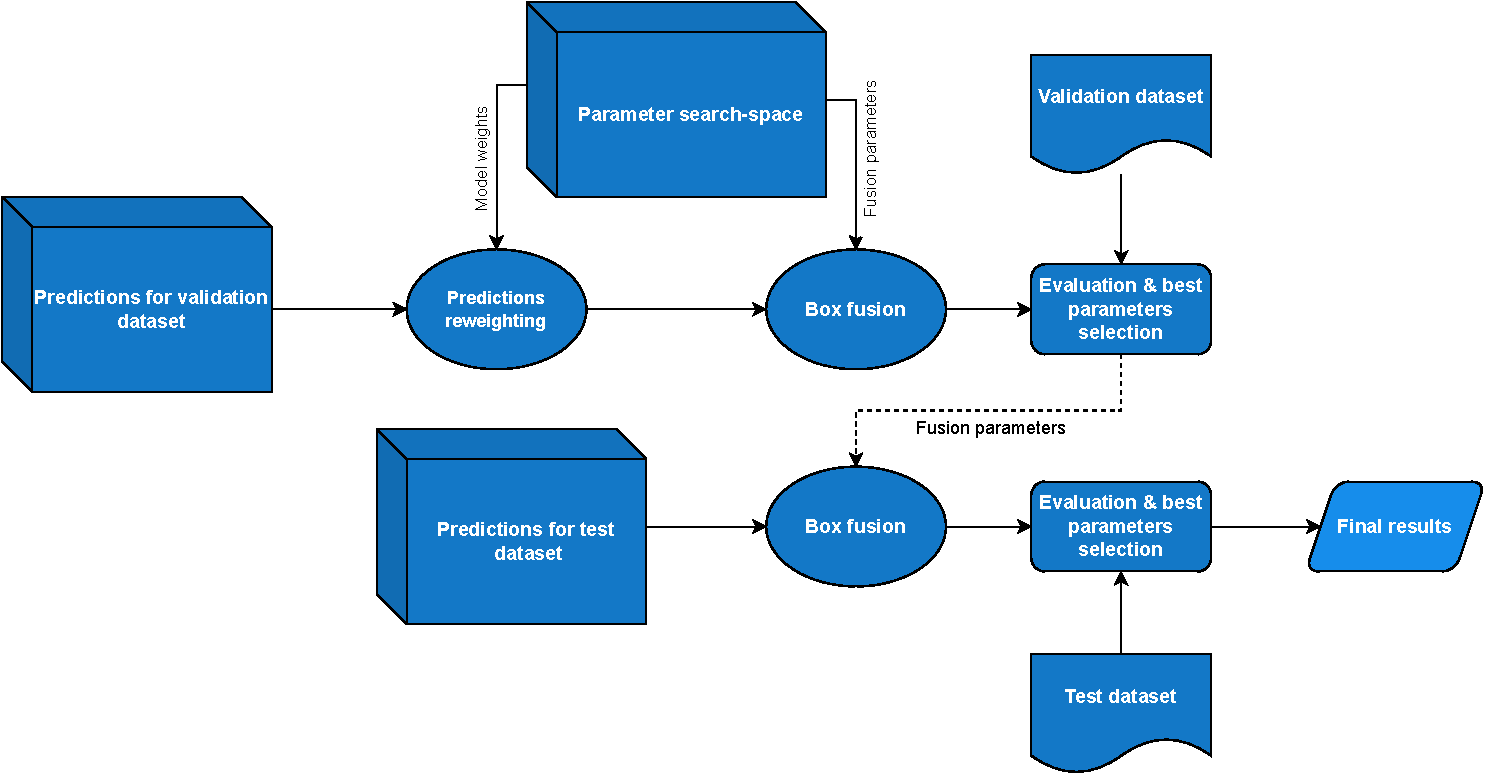
\includegraphics[width=\linewidth]{images/ensemble_search_diag.drawio.pdf}
    \caption{Schematics of the search of hyper-parametrs and weights for ensembling}
    \label{fig:diag:ense_search}
\end{figure}

\begin{figure}
    \centering
    \begin{lstlisting}[language=json, numbers=none]
   {"filename" : {
       "bboxes" : [[x1, y1, x2, y2],...],
       "labels": [l1, l2,...],
       "scores": [s1, s2,...],
       "stage" : "test" / "val" / "train"
       },
    "filename2" : {...},
    ...
   }
\end{lstlisting}
    \caption{Structure of the data in .json file used to store model predictions}
    \label{fig:predictions_json}
\end{figure}

\subsection{Assesing importance of different models in ensembling}
To get an insight into what affects the performance of model ensembling we compare the following: Ensemble of multiple models with the same architecture and backbone, ensemble of models with the same architecture and different backbones, ensemble of different architectures.



\subsubsection{The same architecture and backbone}
We selected a total of eight pretrained YOLOv5 model with medium size backbone. All those model were trained on stage five dataset.
